\part{NEA}

\section{Formale Definition}

$A=(Q,\Sigma,\delta,q_{i},F)$

Q ist die Menge aller möglichen Zustände = $\{q_0,q_1,...,q_{n-1}\}$

$\Sigma$ ist die Menge aller möglichen Eingaben = $\{e_0,e_{1},...,e_{n-1}\}$

F ist die Menge aller möglichen Endzustände = $F\subseteq Q$

$q_{i}\epsilon Q$ der Endzustand ist in Q enthalten

$\delta:Q \times (\Sigma \bigcup \{\epsilon\}) \rightarrow 2^Q$

%$\{\delta_1(q,a)\}$ für alle q $\epsilon$ $\Sigma$ und a $\epsilon$ $\Sigma$, für die $\delta_1(q,a)$ definiert ist 

\[
 x =
  \begin{cases}
   \{\delta_1(q_i,a)\} & \text{ für alle q } \epsilon \Sigma \text{ und a } \epsilon \Sigma \text{, für die } \delta_1(q_i,a) \text{ definiert ist} \\
	\emptyset & \text{ sonst}
  \end{cases}
\]

Es muss bei der Definition explizit darauf hingewiesen werden welcher Automatentyp vorhanden ist (DEA/NEA).

\section*{Beispiel:}\mbox{} \\


\section{Zustandsdiagramm}

\paragraph{Beispiel:}\mbox{} \\

\begin{tikzpicture}[>=stealth',shorten >=1pt,auto,node distance=2.5 cm, scale = 1, transform shape]

\node[initial,state] 				(A)                          {$q_0$};
\node[state] 						(B) [right of=A]             {$q_1$};
\node[state] 						(C) [right of=B]             {$q_2$};
\node[state,accepting] 				(D) [right of=A]             {$q_3$};
\node[state] 						(E) [right of=A]             {$q_4$};
\node[state] 						(F) [above of=E]             {$q_5$};

\path[->] 	(A) edge [right, above]	   		node [align=center]  {$ a $} 	(B)
			(A) edge [right, above]   		node [align=center]  {$ a $} 	(C)
			(A) edge [right, above]   		node [align=center]  {$ a,b $} 	(D)
			(A) edge [right, above]   		node [align=center]  {$ b $} 	(F)

			(B) edge [right, above, loop]   node [align=center]  {$ a $} 	(B)
			(B) edge [right, above, loop]   node [align=center]  {$ a $} 	(C)
			(B) edge [right, above, loop]   node [align=center]  {$ a $} 	(D)

			(E) edge [right, above, loop]   node [align=center]  {$ b $} 	(D)
			(E) edge [right, above, loop]   node [align=center]  {$ b $} 	(F)

			(F) edge [right, above, loop]   node [align=center]  {$ b $} 	(E)
			;      		

\end{tikzpicture}

\section{Automatentafel}

\paragraph{Beispiel:}\mbox{} \\
\begin{tabular}{ l | c r }
  $\delta$ 		& a 	& b \\
  \hline
  $\rightarrow q_0$ 	& $\{q_1,q_2,q_3\}$ & $\{q_3,q_5\}$ \\
  $q_1$				& $\{q_1,q_2,q_3\}$	& $\emptyset$ \\
  $q_2$				& $\emptyset$		& $\emptyset$ \\
  $emptybox q_3$	& $\emptyset$		& $\emptyset$ \\
  $q_4$				& $\emptyset$		& $\{q_5,q_3\}$ \\
  $q_5$				& $\emptyset$		& $\{q_4\}$
\end{tabular}

\section{Umwandlung $\epsilon$-NEA in NEA}

$\epsilon$-Übergänge sind Zustandsübergänge ohne Eingabe, denn $\epsilon$ bedeutet, dass man keine Eingabe tätigt.

\section{Umwandlung NEA $\rightarrow$ DEA}

\begin{table}[!htb]    
    \begin{minipage}{.5\linewidth}
      \caption{Ursprungs-NEA}
      \centering
      \begin{tabular}{ l | c r }
		  $\delta$ 		& a 	& b \\
		  \hline
		  $\rightarrow q_0$ 	& $\{q_1,q_2,q_3\}$ & $\{q_3,q_5\}$ \\
		  $q_1$					& $\{q_1,q_2,q_3\}$	& $\emptyset$ \\
		  $q_2$					& $\emptyset$		& $\emptyset$ \\
		  $emptybox q_3$		& $\emptyset$		& $\emptyset$ \\
		  $q_4$					& $\emptyset$		& $\{q_5,q_3\}$ \\
		  $q_5$					& $\emptyset$		& $\{q_4\}$
		\end{tabular}
    \end{minipage}%
    \begin{minipage}{.5\linewidth}
      \centering
        \caption{Äquivalenter DEA}
        \begin{tabular}{ l | c r }
		  $\delta$ 		& a 	& b \\
		  \hline
		  $\rightarrow q_0$ 	& $\{q_1,q_2,q_3\}$ & $\{q_3,q_5\}$ \\
		  $\Box \{q_1,q_2,q_3\}$		& $\{q_1,q_2,q_3\}$	& $\emptyset$ \\
		  $\Box \{q_3,q_5\}$	& $\emptyset$		& $\{q_4\}$ \\
		  $q_4$					& $\emptyset$		& $\{q_5,q_3\}$ \\	
		  						&					& \\
		  						&					& \\
		\end{tabular}
    \end{minipage} 
\end{table}

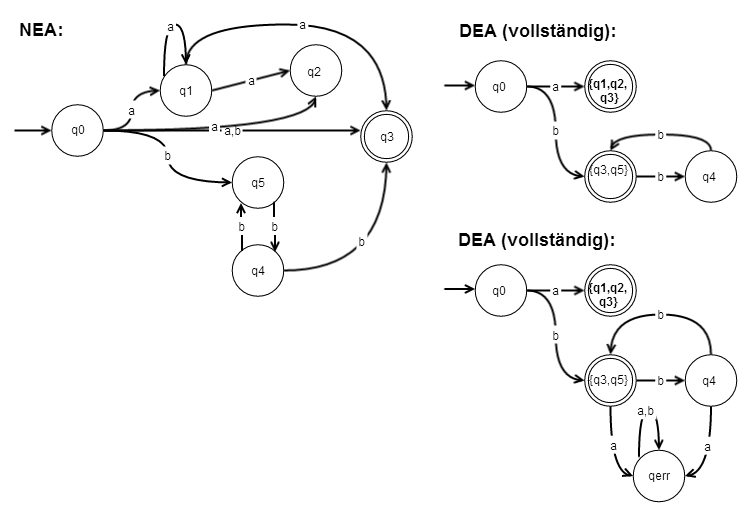
\includegraphics[width=\textwidth]{nea2dea}